%%%%%%%%%%%%%%%%%%%%%%%%%%%%%%%%%%%
%This is the LaTeX ARTICLE template for RSC journals
%Copyright The Royal Society of Chemistry 2016
%%%%%%%%%%%%%%%%%%%%%%%%%%%%%%%%%%%

\documentclass[twoside,twocolumn,9pt]{article}
\usepackage{extsizes}
\usepackage[super,sort&compress,comma]{natbib} 
\usepackage[version=3]{mhchem}
\usepackage[left=1.5cm, right=1.5cm, top=1.785cm, bottom=2.0cm]{geometry}
\usepackage{balance}
\usepackage{mathptmx}
\usepackage{sectsty}
\usepackage{graphicx} 
\usepackage{lastpage}
\usepackage[format=plain,justification=justified,singlelinecheck=false,font={stretch=1.125,small,sf},labelfont=bf,labelsep=space]{caption}
\usepackage{float}
\usepackage{fancyhdr}
\usepackage{fnpos}
\usepackage[english]{babel}
\addto{\captionsenglish}{%
  \renewcommand{\refname}{Notes and references}
}
\usepackage{array}
\usepackage{droidsans}
\usepackage{charter}
\usepackage[T1]{fontenc}
\usepackage[usenames,dvipsnames]{xcolor}
\usepackage{setspace}
\usepackage[compact]{titlesec}
\usepackage{hyperref}
%%%Please don't disable any packages in the preamble, as this may cause the template to display incorrectly.%%%


\usepackage{epstopdf}%This line makes .eps figures into .pdf - please comment out if not required.

\definecolor{cream}{RGB}{222,217,201}

\begin{document}

\pagestyle{fancy}
\thispagestyle{plain}
\fancypagestyle{plain}{
%%%HEADER%%%
\renewcommand{\headrulewidth}{0pt}
}
%%%END OF HEADER%%%

%%%PAGE SETUP - Please do not change any commands within this section%%%
\makeFNbottom
\makeatletter
\renewcommand\LARGE{\@setfontsize\LARGE{15pt}{17}}
\renewcommand\Large{\@setfontsize\Large{12pt}{14}}
\renewcommand\large{\@setfontsize\large{10pt}{12}}
\renewcommand\footnotesize{\@setfontsize\footnotesize{7pt}{10}}
\makeatother

\renewcommand{\thefootnote}{\fnsymbol{footnote}}
\renewcommand\footnoterule{\vspace*{1pt}% 
\color{cream}\hrule width 3.5in height 0.4pt \color{black}\vspace*{5pt}} 
\setcounter{secnumdepth}{5}

\makeatletter 
\renewcommand\@biblabel[1]{#1}            
\renewcommand\@makefntext[1]% 
{\noindent\makebox[0pt][r]{\@thefnmark\,}#1}
\makeatother 
\renewcommand{\figurename}{\small{Fig.}~}
\sectionfont{\sffamily\Large}
\subsectionfont{\normalsize}
\subsubsectionfont{\bf}
\setstretch{1.125} %In particular, please do not alter this line.
\setlength{\skip\footins}{0.8cm}
\setlength{\footnotesep}{0.25cm}
\setlength{\jot}{10pt}
\titlespacing*{\section}{0pt}{4pt}{4pt}
\titlespacing*{\subsection}{0pt}{15pt}{1pt}
%%%END OF PAGE SETUP%%%

%%%FOOTER%%%
\fancyfoot{}
\fancyfoot[LO,RE]{\vspace{-7.1pt}
\includegraphics[height=9pt]{head_foot/LF}}
\fancyfoot[CO]{\vspace{-7.1pt}\hspace{13.2cm}
\includegraphics{head_foot/RF}}
\fancyfoot[CE]{\vspace{-7.2pt}\hspace{-14.2cm}
\includegraphics{head_foot/RF}}
\fancyfoot[RO]{\footnotesize{\sffamily{1--\pageref{LastPage} ~\textbar  \hspace{2pt}\thepage}}}
\fancyfoot[LE]{\footnotesize{\sffamily{\thepage~\textbar\hspace{3.45cm} 1--\pageref{LastPage}}}}
\fancyhead{}
\renewcommand{\headrulewidth}{0pt} 
\renewcommand{\footrulewidth}{0pt}
\setlength{\arrayrulewidth}{1pt}
\setlength{\columnsep}{6.5mm}
\setlength\bibsep{1pt}
%%%END OF FOOTER%%%

%%%FIGURE SETUP - please do not change any commands within this section%%%
\makeatletter 
\newlength{\figrulesep} 
\setlength{\figrulesep}{0.5\textfloatsep} 

\newcommand{\topfigrule}{\vspace*{-1pt}% 
\noindent{\color{cream}\rule[-\figrulesep]{\columnwidth}{1.5pt}} }

\newcommand{\botfigrule}{\vspace*{-2pt}% 
\noindent{\color{cream}\rule[\figrulesep]{\columnwidth}{1.5pt}} }

\newcommand{\dblfigrule}{\vspace*{-1pt}% 
\noindent{\color{cream}\rule[-\figrulesep]{\textwidth}{1.5pt}} }

\makeatother
%%%END OF FIGURE SETUP%%%

%%%TITLE, AUTHORS AND ABSTRACT%%%
\twocolumn[
  \begin{@twocolumnfalse}
{
\includegraphics[height=30pt]{head_foot/journal_name}\hfill\raisebox{0pt}[0pt][0pt]{
\includegraphics[height=55pt]{head_foot/RSC_LOGO_CMYK}}\\[1ex]

\includegraphics[width=18.5cm]{head_foot/header_bar}}\par
\vspace{1em}
\sffamily
\begin{tabular}{m{4.5cm} p{13.5cm} }


\includegraphics{head_foot/DOI} & \noindent\LARGE{\textbf{In Silico Screening of Metal-Organic Frameworks for CO\textsubscript{2} Photo-Hydrogenation}} \\%Article title goes here instead of the text "This is the title"
\vspace{0.3cm} & \vspace{0.3cm} \\

 & \noindent\large{Moin Khwaja\textit{$^{a}$}, Adrian Loy Chun Minh\textit{$^{ab}$}, and Takuya Harada\textit{$^{a\ast}$~}} \\%Author names go here instead of "Full name", etc.

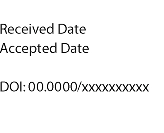
\includegraphics{head_foot/dates} & \noindent\normalsize{Metal-organic frameworks (MOFs) are a promising class of materials that can be used as a catalyst for photo-hydrogenation to convert CO\textsubscript{2} to fuel by virtue to their nanoscale design featuring high surface area, abundant active metal sites, and ability to host dispersed co-catalysts. However due to the vast combination of materials possible and general fragility of MOFs, experimental identification of catalytic material is non-trivial. To aid in finding optimal catalytic candidates, we implement a multi-tiered high-throughput screening of 20,375 in silico MOFs for their porosity (\(\ge \)4.5\AA), light adsorption (1.7-3.5 eV), aqueous stability, and solvent removal stability. The 24 passing materials were evaluated by density functional theory (DFT) using proton-coupled electron transfer pathway for CO\textsubscript{2} to CH\textsubscript{4}. Of the eight thermodynamically favorable materials, three materials have been previously synthesized and the material precursors were analyzed for their material cost and life-cycle analysis showing Mg-MOF-74 with the lowest material cost (\$15.11 per gram) and environmental impact. The five novel materials using aluminum and zinc-based frameworks with pore diameters ranging from 4.7 to 21.6 Å, are presented for novel experimental realization.} \\

\end{tabular}

 \end{@twocolumnfalse} \vspace{0.6cm}

  ]
%%%END OF TITLE, AUTHORS AND ABSTRACT%%%

%%%FONT SETUP - please do not change any commands within this section
\renewcommand*\rmdefault{bch}\normalfont\upshape
\rmfamily
\section*{}
\vspace{-1cm}


%%%FOOTNOTES%%%

\footnotetext{\textit{$^{a}$~Department of Chemical Science and Engineering, Institute of Science Tokyo, Meguro, Tokyo 152-8550, Japan.}}

\footnotetext{\textit{$^{b}$~Department of Chemical Engineering, The University of Melbourne, Parkville, Victoria 3010, Australia.}}
%Please use \dag to cite the ESI in the main text of the article.
%If you article does not have ESI please remove the the \dag symbol from the title and the footnotetext below.
\footnotetext{$^{\ast}$~Tel: +81-3-5734-3292; E-mail: harada.t.2871@m.isct.ac.jp}
%Please use \dag to cite the ESI in the main text of the article.
%If you article does not have ESI please remove the the \dag symbol from the title and the footnotetext below.
%\footnotetext{\dag~Supplementary Information available: [details of any supplementary information available should be included here]. See DOI: 00.0000/00000000.}
%additional addresses can be cited as above using the lower-case letters, c, d, e... If all authors are from the same address, no letter is required

%%%END OF FOOTNOTES%%%

%%%MAIN TEXT%%%%
\section{Introduction}

Over the past several decades, significant amounts of carbon dioxide has been released into the atmosphere as a result of fossil fuel combustion, leading to a rise in global warming\cite{hansen_target_2008, choi_research_2008}. As new green technologies are developed to decarbonize a large portions of global industry, several sectors remain difficult to entirely convert\cite{welsby_unextractable_2021}. In order to ramp down the net positive carbon dioxide release in these sectors, the idea of a circular carbon fuel economy\cite{kirchherr_conceptualizing_2017} has been proposed, where CO\textsubscript{2} is utilized to create carbon neutral fuels. To support this, research is being done on methods of converting CO\textsubscript{2} back into hydrocarbon fuels, closing the circular carbon economy\cite{roy_toward_2010}.

\par

To convert CO\textsubscript{2}, catalytic conversion has been established as one of the most promising approach to economically reaching set sustainability goals\cite{clark_circular_2016}. Major catalytic approaches include electrocatalysis\cite{segets_accelerating_2023}, photocatalysis\cite{alli_photocatalysts_2023}, and thermal-catalysis\cite{wen_recent_2025}. Despite advances in the field, efficiently cleaving the C=O bond continues to be a challenge with reactions rates remaining sluggish\cite{jin_advances_2021, zhao_progress_2017}. 

\par

Thermal-catalytic conversion of CO\textsubscript{2} uses heat to promote the breakage of bonds\cite{jadhav_catalytic_2014, roy_thermochemical_2018}. When paired with renewable hydrogen, hydrogenation of CO\textsubscript{2} occurs, resulting in products depending on the reaction pathway, such as CO through the reverse water-gas shift or methane/methanol by Fischer-Tropsch\cite{olah_chemical_2017}. However, this high heat required to break the bonds can result in a net-positive carbon emission, in addition to creating a harsh reaction environment that deteriorates the catalysts\cite{ye_design_2025}. CO\textsubscript{2} photocatalytic conversion has been of high interest as an "artificial photosynthetic route"\cite{alli_photocatalysts_2023}, however reactions suffer from low output compared to other catalytic methods\cite{liao_challenges_2024}. 

\par

Photo-hydrogenation combines the advantages of both methods to accelerate the overall catalytic process by using light to promote charge excitation and separation, lowering the required heat to carry out the reaction\cite{guo_state---art_2022, li_fe-based_2021}. Additionally, photo-hydrogenation can harness the full solar spectrum, improving the efficiency of the process\cite{long_efficient_2015}. 

\par

Recently, metal-organic frameworks (MOFs) have emerged as highly customizable material as an absorbent, membrane, and as a catalyst\cite{zhou_introduction_2012, furukawa_chemistry_2013, yaghi_reticular_2003}. They have also shown promise as a catalyst for CO\textsubscript{2} hydrogenation by virtue of their high porosity, large surface area, abundant metal sites, and the ability to host co-catalysts within their framework system\cite{ye_organic-inorganic_2023, zhai_photo-thermal_2024, stanley_analysis_2024, wang_dual_2026}. This porous structure is created by a combination of metal nodes, known as secondary building units (SBU), and organic ligands, known as linkers. This highly tailor-able combination allows for efficient distribution of catalytic sites that are accessible to molecules that can fit within the porosity of the material\cite{doi:10.1126/science.1230444, maina_metal_2017, li_integration_2014, dou_hierarchically_2020}.

\par

The immense array of possible material combinations has created challenges in finding target materials, as it becomes experimentally intensive to synthesize and test each material. To accelerate this search, computational material generation and high-throughput screenings have been implemented to quickly screen materials for key target properties\cite{li_high-throughput_2016, hai_high-throughput_2022, liu_high-throughput_2025, tan_high_2025, kum_high-throughput_2025,khwaja_high-throughput_2024, anselmi_accelerating_2026, morandi_end--end_2026, hu_identifying_2025, wang_silico_2024}. In recent years, advances in available computing power has allowed for use of large-scale first-principles simulations to create open-source databases for material exploration. The Materials Project\cite{jain_commentary_2013, horton_accelerated_2025}, part of the Materials Genome Initiative\cite{de_pablo_materials_2014, de_pablo_new_2019}, leveraged high-throughput density functional theory (DFT) calculations to create a materials database populated with materials structures and electronic energies. Together with machine-learning models to target harder to predict properties such as thermal stability\cite{nandy_mofsimplify_2022} and water stability\cite{batra_prediction_2020, terrones_metalorganic_2024}, efficient high-throughput methods can be made to find materials for targeted use cases. 

\par

In this work, we present an efficient high-throughput screening method to search for metal-organic frameworks that are candidates for CO\textsubscript{2} hydrogenation without the need of expensive and time-consuming experimental work. we follow a broad database search, machine-learning screening, then implement reaction energy screening using DFT methods. Material cost (MC) and life-cycle analysis (LCA) are then conducted on the final passing materials with experimental synthesis pathways available to show highly scalable materials. 

\section{Methodologies}
\subsection{High-Throughput Screening}

Several screening stages were required to ensure the passing materials are suitable for CO\textsubscript{2} hydrogenation. The Materials Project MOF Explorer\cite{rosen_high-throughput_2022} was used as the main database screened in this study. Populated by the Quantum MOFs (QMOF) database\cite{rosen_machine_2021}, MOF Explorer supplied the materials CIF structure files, material porosity\cite{willems_algorithms_2012}, and Perdew-Burke-Ernzerhof (PBE) calculated band gap energies\cite{perdew_generalized_1996}. Table S1 shows the database version used along with DFT methods implemented for energy calculations. Figure 1 describes the overall screening methodology.

\begin{figure}[h]
\centering
  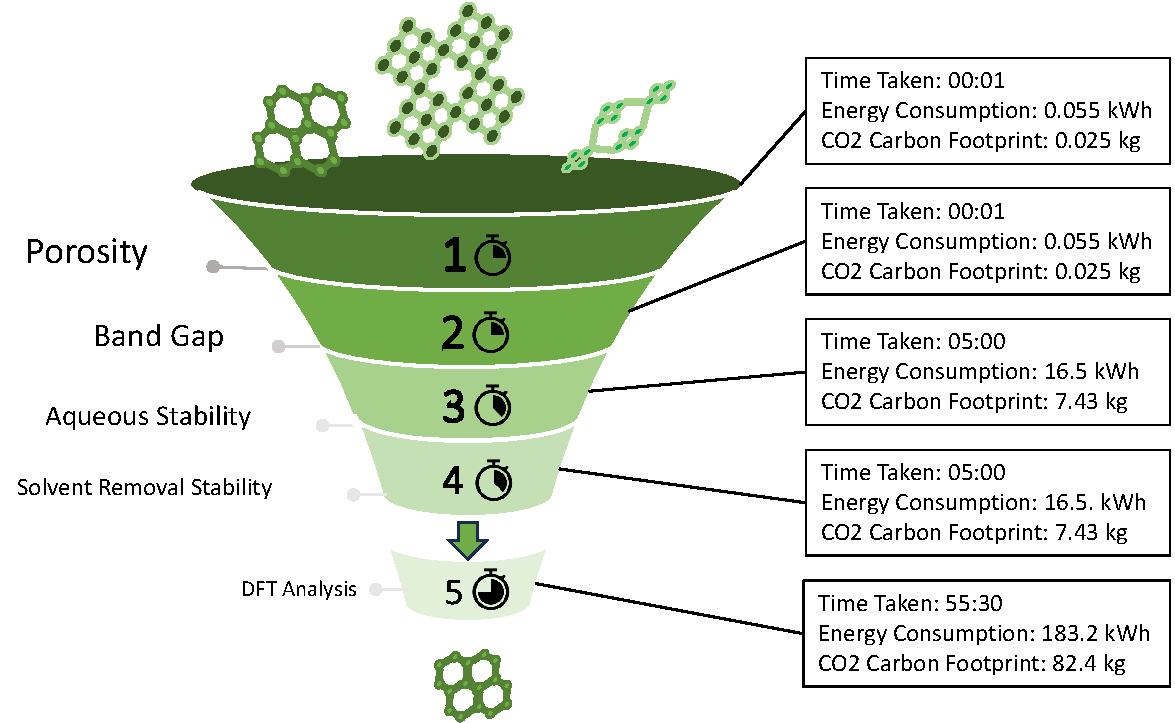
\includegraphics[height=5cm]{figure1c.pdf}
  \caption{Workflow for the metal-organic framework screening method along with generalized time per step. High-throughput screening is done for porosity, band gap, aqueous stability, and solvent removal stability. DFT reaction energies are then calculated for the passing materials. Time taken per each step is noted along with the estimated energy used by one Tsubame4.0 node running the calculation}
  \label{fgr:example}
\end{figure}

\begin{figure*}
 \centering
 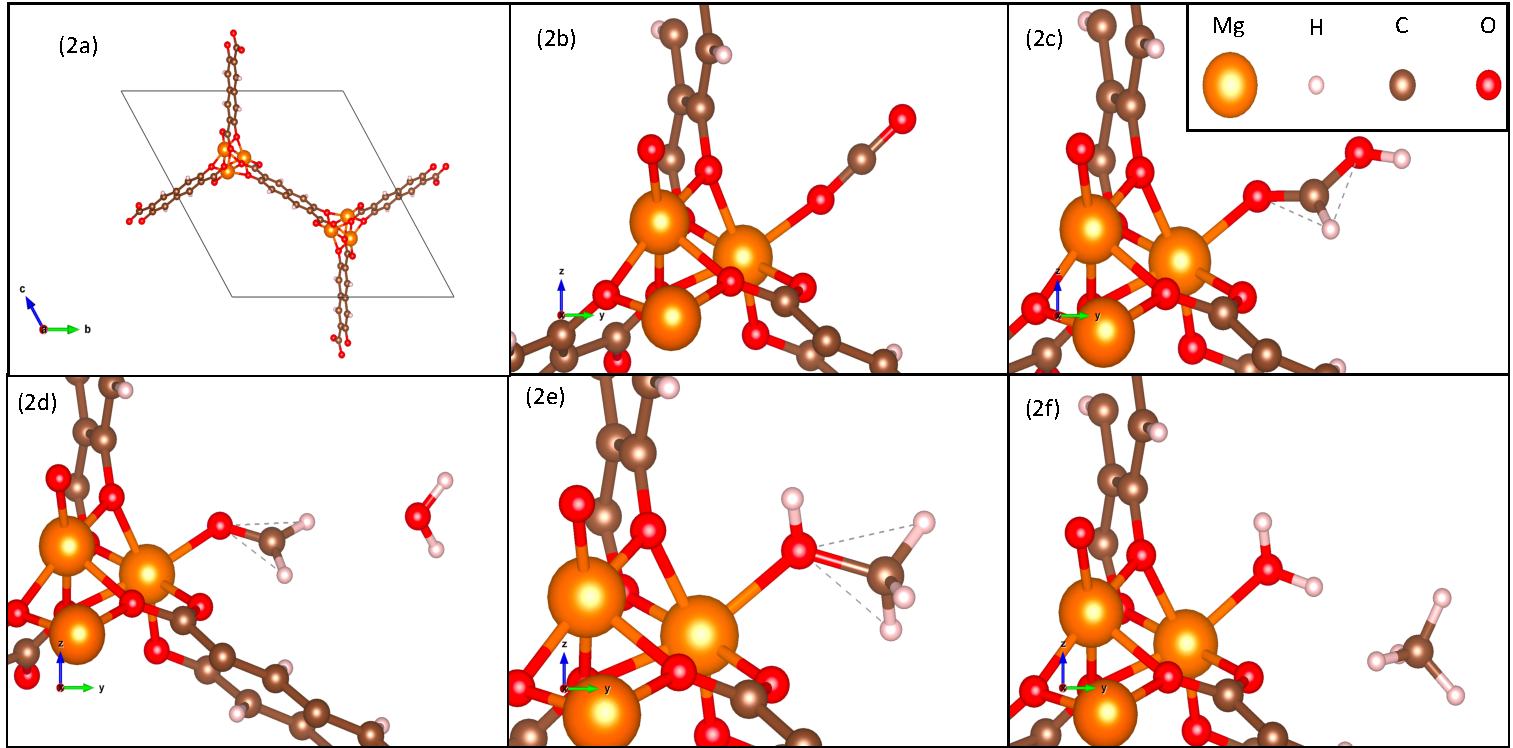
\includegraphics[height=8cm]{figure2d.pdf}
 \caption{DFT Simulations of the catalytic CO\textsubscript{2} reduction mechanism. (2a) Initial optimized geometry of the metal-organic framework (MOF) unit cell, obtained via geometry relaxation of the CIF structure provided by the Materials Project. The framework features an active metal cluster center coordinated by organic linkers.(2b) Structural configuration following the initial adsorption of a CO\textsubscript{2} molecule onto the active metal site, demonstrating the formation of the critical node–CO\textsubscript{2} intermediate.(2c, 2d) Sequential hydrogenation steps illustrating the addition of 2 hydrogen atoms, moved into place by geometry optimization. The transition from (2c) to (2d) involves geometry optimization leading to the cleavage of the C–O bond and the formation of a water molecule (H\textsubscript{2}O), which is subsequently removed from the active site.(2e) Further hydrogenation of the remaining carbonaceous intermediate, showing the progressive addition of hydrogen atoms to the metal-bound carbon center.(2f) Final reaction stage depicting the addition of the remaining hydrogen atoms, resulting in the successful release of methane (CH\textsubscript{4}) and the secondary H\textsubscript{2}O molecule, thereby regenerating the catalytic active site for subsequent cycles.}
 \label{fgr:example2col}
\end{figure*}
\par

The first tier, porosity, allows for the CO\textsubscript{2} molecule to access the large surface area inside the MOF, reaching the active sites where catalytic conversion can take place\cite{gao_coordination_2017}. To ensure that this can happen, the porosity needs to be larger than the starting molecules entering and the product leaving the MOFs pores. Previous screening methodologies implement a bottom limit of 3.3 Angstroms\cite{hai_high-throughput_2022}, however this may lead to CO\textsubscript{2} capture as CO\textsubscript{2} absorption on the active sites block the movement of other CO\textsubscript{2} molecules\cite{li_porous_2020}. To ensure that the CO\textsubscript{2} and products can freely move through the pores, a pore diameter was set to 4.5 Angstroms or larger. 

\par

The second tier, band gap, screens for the electronic structure of the MOFs. The electronic structure of MOFs differs from other materials as each node and ligand has varying electronic properties\cite{usman_semiconductor_2017} and can interact with each other through metal-to-metal, metal-to-ligand, and ligand-to-ligand charge transfers, boosting the catalytic ability of the material\cite{li_metal-organic_2019}. The general semiconducting band structure of the MOFs is then referred to as the highest occupied molecular orbital (HOMO) and the lowest unoccupied molecular orbital (LUMO)\cite{perdew_generalized_1996}. To calculate the band gap of the MOFs, the QMOF database carried out high-throughput DFT calculations at the PBE-D3\cite{grimme_dispersion-corrected_2016} level of theory. Additional DFT details for the QMOF database are written in table S2. While the speed of calculations has increased, PBE calculations have historically underestimated the band gap of the materials when compared to experimental results\cite{rosen_high-throughput_2022}. Fumanal et al. demonstrated this for a dataset of 132 MOFs spanning a diverse set of metal nodes and ligand types and found that an empirical shift of 0.85 eV would allow PBE band gaps to yield reasonable agreement with experimentally obtained band gaps\cite{fumanal_charge_2020}. While the estimation may not account for all MOFs possible, a relaxed screening window was targeted to allow that materials near the boundary have a margin of error. To absorb sunlight to assist in the hydrogenation process, the materials require a band gap from 1.7 eV to 3.5 eV, with the empirical shift, we screen for materials for PBE calculated band gaps of 0.85 eV to 2.65 eV. 

\par

The third tier, aqueous stability, predicts the materials stability in the presence of water. MOFs are particularly sensitive to humid conditions as they can have weak metal coordination bonds\cite{an_stability_2024}. The metal coordination can be replaced by water molecules leading to the MOFs decomposition and collapse\cite{yu_topological_2021}. Several machine learning models have now been created and implemented to screen a MOFs ability to remain stable by comparing its structure to structures of MOFs that have been exposed to water. We use a model developed by Terrones et al.\cite{terrones_metalorganic_2024} based on the model developed by Batra et al.\cite{batra_prediction_2020} Experimental MOF CIF files were parsed through a molecular fingerprinting process, revised autocorrelation (RACs)\cite{noauthor_rdkit_nodate}, to generate computational descriptors. This model was trained on 1092 MOFs, and resulted in a model with 0.84 prediction accuracy on the testing dataset. 

\par

The fourth tier, stability upon solvent removal/evacuation, looks at the MOFs ability to remain standing/stable once removed from its synthesis solvent. As MOFs are porous materials, the synthesis solvent can fill the pores and act as an inner support to keep the structure standing. upon removal of the solvent by filtration/drying, the material can collapse in on itself\cite{an_stability_2024}. We use MOFsimplify's stability prediction model to predict the MOFs structural stability. Built on a model developed by Nandy et al.\cite{nandy_mofsimplify_2022, nandy_using_2021}, 2000 experimental MOF's stability data were found and analyzed by natural language processing. These structures were processed again by RACs and used to correlate structure to stability. 

\par

Lastly, we analyze each MOF's CO\textsubscript{2} adsorption potential by scanning each material for open metal sites (OMS)\cite{li_mof-based_2020}. OMS is an important feature of a MOF where an unsaturated metal site is available for bond formation with a reactant molecule\cite{hai_high-performance_2018}. To detect is an OMS is present, we implement an open metal searching algorithm developed by Chung et al.\cite{chung_advances_2019} Using Zeo++\cite{willems_algorithms_2012, martin_construction_2014}, a porous material analysis software, the algorithm searches for metal atoms and determines the coordination sphere around it. 

\subsection{Density Functional Theory}



To validate the materials for CO\textsubscript{2} reduction resulting in CH\textsubscript{4} on candidate MOFs, we follow the methodology described by McCarver et al.\cite{mccarver_catalyst_2023}. We examine the reaction steps as shown in Figure 2. Using the cluster models provided by the Materials Project, each step of the reaction was carried out via a proton-coupled electron transfer (PCET) mechanism to maintain a charge neutrality within the complex\cite{verma_mechanism_2015}. The adsorption energy for each intermediate along the reaction coordinate is given by equation 1:
\begin{equation}E_{\text{ads}} = E_{\text{MOF+intermediate}} - (E_{\text{intermediate}} + E_{\text{MOF}}^{n-1})\end{equation}
where E\textsubscript{MOF+intermediate} is the total energy of the MOF with the adsorbed intermediate at step \textit{n}, E\textsubscript{intermediate} is the energy of the isolated intermediate species, and E\textsubscript{MOF}\textsuperscript{n-1} is the energy of the MOF in the state resulting from the preceding reaction step. For the initial CO\textsubscript{2} adsorption, E\textsubscript{MOF}\textsuperscript{n-1} corresponds to the bare optimized MOF cluster.

\par

The computational density functional theory (DFT) work was carried out using the QUICKSTEP module\cite{vandevondele_quickstep_2005} of the CP2K software package\cite{kuhne_cp2k_2020} with the Gaussian and Plane Waves (GPW) method\cite{lippert_hybrid_1997}. The Perdew-Burke-Ernzerhof (PBE) exchange-correlation functional\cite{perdew_generalized_1996} was used in conjunction with the DFT-D3 dispersion correction\cite{grimme_dispersion-corrected_2016}. The MOLOPT basis set was used for all atoms\cite{vandevondele_gaussian_2007}, along with Goedecker-Teter-Hutter (GTH) pseudopotentials\cite{goedecker_separable_1996} to describe the core electrons. A cutoff energy of 450 Ry was applied with a relative cutoff of 60 Ry using four multi-grids. The self-consistent field (SCF) calculations\cite{kohn_self-consistent_1965} used the orbital transformation (OT) method\cite{vandevondele_efficient_2003} with direct inversion in the iterative subspace (DIIS) minimizer\cite{pulay_convergence_1980}. SCF convergence thresholds were set to 1.0e\textsuperscript{-5} atomic units (AU). Geometry optimizations were done by using the Broyden-Fletcher-Goldfarb-Shanno (BFGS) algorithm\cite{nocedal_numerical_2006} with the convergence criteria set to 3.0e\textsuperscript{-3}. Materials were deemed thermodynamically favorable if all sequential PCET steps along the reaction pathway were exothermic relative to the preceding intermediate. Individual molecule energies are shown in table S3. We note that this screening evaluates thermodynamic driving forces only; kinetic barriers between intermediates, which would require transition state calculations (e.g., CI-NEB), comparisons of our thermodynamic screening method with deeper computational/experimental analysis on passing materials with literature references are discussed in Section 4.



\subsection{Material Cost and Life Cycle Analysis}

Material cost and life cycle analysis were done on all materials that have been experimentally synthesized and passed the high-throughput screening tiers. 

A simplified material cost analysis was done based on direct material costs  with the functional unit set to 1 gram of product. This analysis focuses on the relative cost comparison based on the synthesis of each catalysts (raw materials and consumables were found in AUD from Sigma-Aldrich\cite{noauthor_sigma-aldrich_nodate} then converted to USD [1 AUD = 0.68 USD], and energy costs are based on the JPY [1 JPY = 0.0063 USD] pricing\cite{oneil_power_2024}). 

\par

Life cycle analysis (LCA) was conducted using Simparo 10.1\cite{noauthor_simapro_nodate} and Ecoinvent 13.1\cite{noauthor_ecoinvent_nodate} using the ISO 14040/14044\cite{finkbeiner_new_2006} and RecCiPe 2016 Midpoint (E) 1.0 methodologies\cite{huijbregts_recipe2016_2017}, with a functional unit defined as the production of 1 gram of material. The analysis focuses on midpoint environmental impact categories under a cradle-to-gate system boundary\cite{finkbeiner_new_2006}. For linkers and precursors lacking publicly available life-cycle inventory data, chemically analogous proxy materials were selected based on comparable functional group densities, molecular weights, and synthetic complexity. In cases where suitable proxies were unavailable, inventories were constructed from upstream raw materials using stoichiometric relationships and literature-reported synthesis routes. These assumptions were applied consistently across all materials to ensure fair benchmarking. 

\section{Results}
\subsection{High-Throughput Screening Results}

Through the QMOF database search, 24 materials were found to fit all the criteria set for stable metal-organic frameworks for photo-hydrogenation. These passing materials are shown in table S4. Figure 3 shows the overall passing rate for each of the screening tiers.



\begin{figure}[h]
\centering
  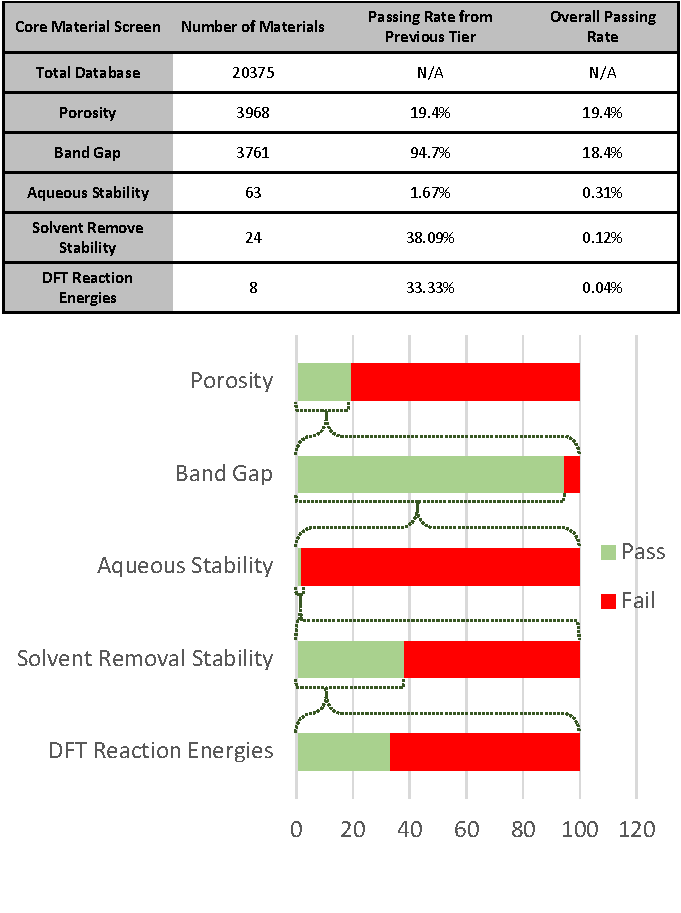
\includegraphics[height=12cm]{figure3c.pdf}
  \caption{Overall passing rate for each of the screening tiers. 3a: passing rate for material porosity. 3b: passing rate for material band gap. 3c: passing rate for aqueous stability. 3d: passing rate for solvent removal stability. 3e: passing rate for DFT reaction energies.}
  \label{fgr:example}
\end{figure}

\begin{figure*}
 \centering
 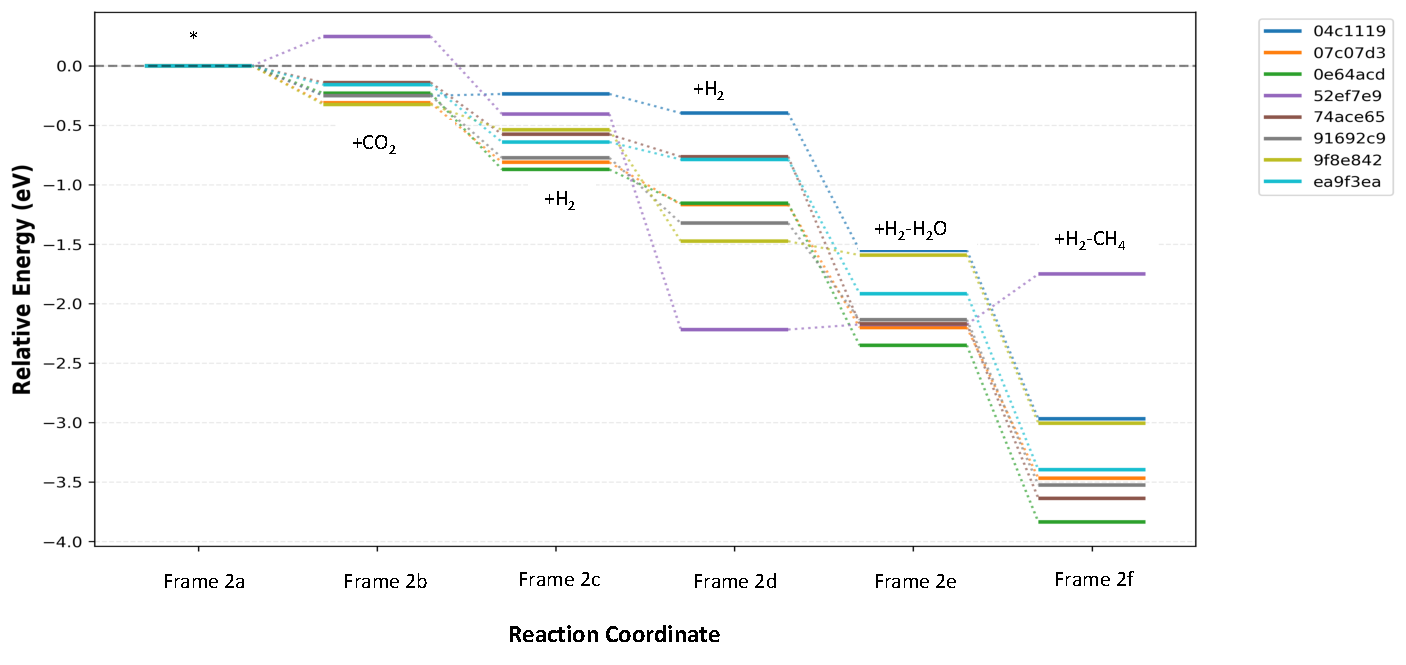
\includegraphics[height=9cm]{figure4c.pdf}
 \caption{Cumulative reaction energies of the passing materials. The reaction coordinates follow the frames shown in figure 2. Energies are shown as relative to the previous steps reaction energy (negative shows the step is exothermic). qmof-52ef7e9 shows slight increase of energy at the addition of CO\textsubscript{2}, however this slight increase should be overcome by the hydrogenation energy.}
 \label{fgr:example2col}
\end{figure*}

The QMOF database search began with 20,375 in silico MOF structures. Figure 3 shows the overall passing rate for each screening tier.
In the first tier, porosity screening with a minimum pore diameter of 4.5 \AA{} removed the majority of the database, with 3,968 MOFs (19.4\%) passing. The second tier, band gap screening for PBE-calculated values between 0.85 eV and 2.65 eV, retained 3,761 of these materials (94.7\% of the previous tier). This is expected as the QMOF database targeted materials with usable electronic structure.
The aqueous stability tier proved to be the most restrictive filter: only 63 of the 3,761 remaining MOFs (1.67\%) were predicted to be stable in humid conditions by the Terrones et al.\cite{terrones_metalorganic_2024} machine learning model. Of these 63 materials, 24 (38.1\%) passed the solvent removal stability screening. The cumulative passing rate from the original database was 0.12\%, yielding 24 candidate MOFs for DFT analysis. The dominant metals among the passing materials were aluminum and zinc, with magnesium and nickel each represented by one MOF variant. Open metal site analysis confirmed that all 24 candidates contained accessible unsaturated metal centers available for CO\textsubscript{2} coordination.

\subsection{Density Functional Theory Results}

First, geometry optimization was done on the 24 passing MOFs. Of these, 2 materials failed to reach SCF convergence even after relaxing the convergence limits, reducing the passing materials to 22. CO\textsubscript{2} was then introduced to each optimized structure next to the open metal site and allowed to relax at the adsorption point. Of the 22 materials, 11 exhibited exothermic CO\textsubscript{2} adsorption energies, indicating thermodynamically favorable adsorption binding. All materials were tested to completion of reaction showing the full thermodynamic profile. 
To calculate the thermodynamic profile of the reaction, the full proton-coupled electron transfer pathway was calculated through the sequential addition of H\textsubscript{2} as described in Section 2.2 and illustrated in Figure 2. Of these, 8 materials exhibited exothermic energies at every step along the reaction coordinate from CO\textsubscript{2} adsorption through to CH\textsubscript{4} release. Figure 4 presents the reaction energy diagrams for these 8 passing materials. All profiles show a consistently downhill energy landscape, with cumulative energy changes ranging from approximately -2.0 eV to -4.0 eV across the full pathway. The initial CO\textsubscript{2} adsorption step and the final hydrogenation step releasing CH\textsubscript{4} and H\textsubscript{2}O generally represent the largest energy changes, while the intermediate hydrogenation steps show more modest exothermic contributions. One exception is qmof-52ef7e9, which exhibits a slight endothermic step at initial CO\textsubscript{2} adsorption before proceeding exothermically through the remaining steps, though this barrier should be overcome by the hydrogenation reaction conditions. Table S5 shows the calculated DFT energies for each step. Table 1 summarizes the 8 final candidates along with their chemical formulas, pore diameters, estimated band gaps, and synthesis status.




\subsection{Material Cost and Life Cycle Analysis Results}

Material cost and life cycle analyses were conducted for the three experimentally synthesized MOFs among the final candidates: qmof-04c1119 (Zn-IRMOF-10), qmof-ea9f3ea (Ni-MOF-74), and qmof-9f8e842 (Mg-MOF-74). Figure 5 presents the estimated synthesis cost per gram of each material, broken down by metal node, organic ligand, solvent, and energy contributions. Mg-MOF-74 exhibited the lowest total cost at approximately \$15 per gram, driven primarily by the low cost of its magnesium precursor (\$0.2), 2,5-dihydroxyterephthalic acid ligand, and low solvent usage. Ni-MOF-74, which shares the same ligand as Mg-MOF-74, showed a comparable total cost with the primary difference arising from the higher cost of the nickel precursor (\$4.37). Zn-IRMOF-10 was the most expensive at approximately \$25 per gram, owing to the cost of its more complex biphenyldicarboxylic acid ligand (\$10) and higher energy requirements during synthesis. Table S6 shows the individual price for the raw materials. 
Figure 6 presents the life cycle analysis results across 18 midpoint environmental impact categories. Mg-MOF-74 showed the lowest environmental impact across nearly all categories due to its lack of solvent use and non-toxic metal node, followed by Ni-MOF-74. Zn-IRMOF-10 exhibited the highest impact in categories including global warming potential, terrestrial ecotoxicity, and fossil resource scarcity, consistent with its more energy-intensive and material-intensive synthesis requirements. Across all three materials, the dominant contributors to environmental impact were solvent use and energy consumption during synthesis rather than the metal precursors themselves. Figure S7 shows the 18 point LCA analysis for each of the materials. 

\begin{figure}[h]
\centering
  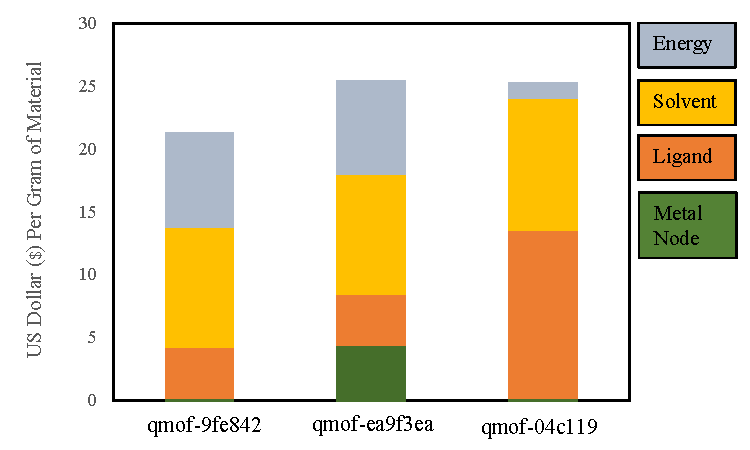
\includegraphics[height=5cm]{figure5f.pdf}
  \caption{Material cost analysis of the previously synthesized qmof-9f8e842, qmof-ea9f3ea, qmof-04c1119and. Main categories include costs of the metal node, ligand, solvent, and energy required during synthesis. Consumables were priced via Sigma-Aldrich Japan}
  \label{fgr:example}
\end{figure}

\begin{figure*}
 \centering
 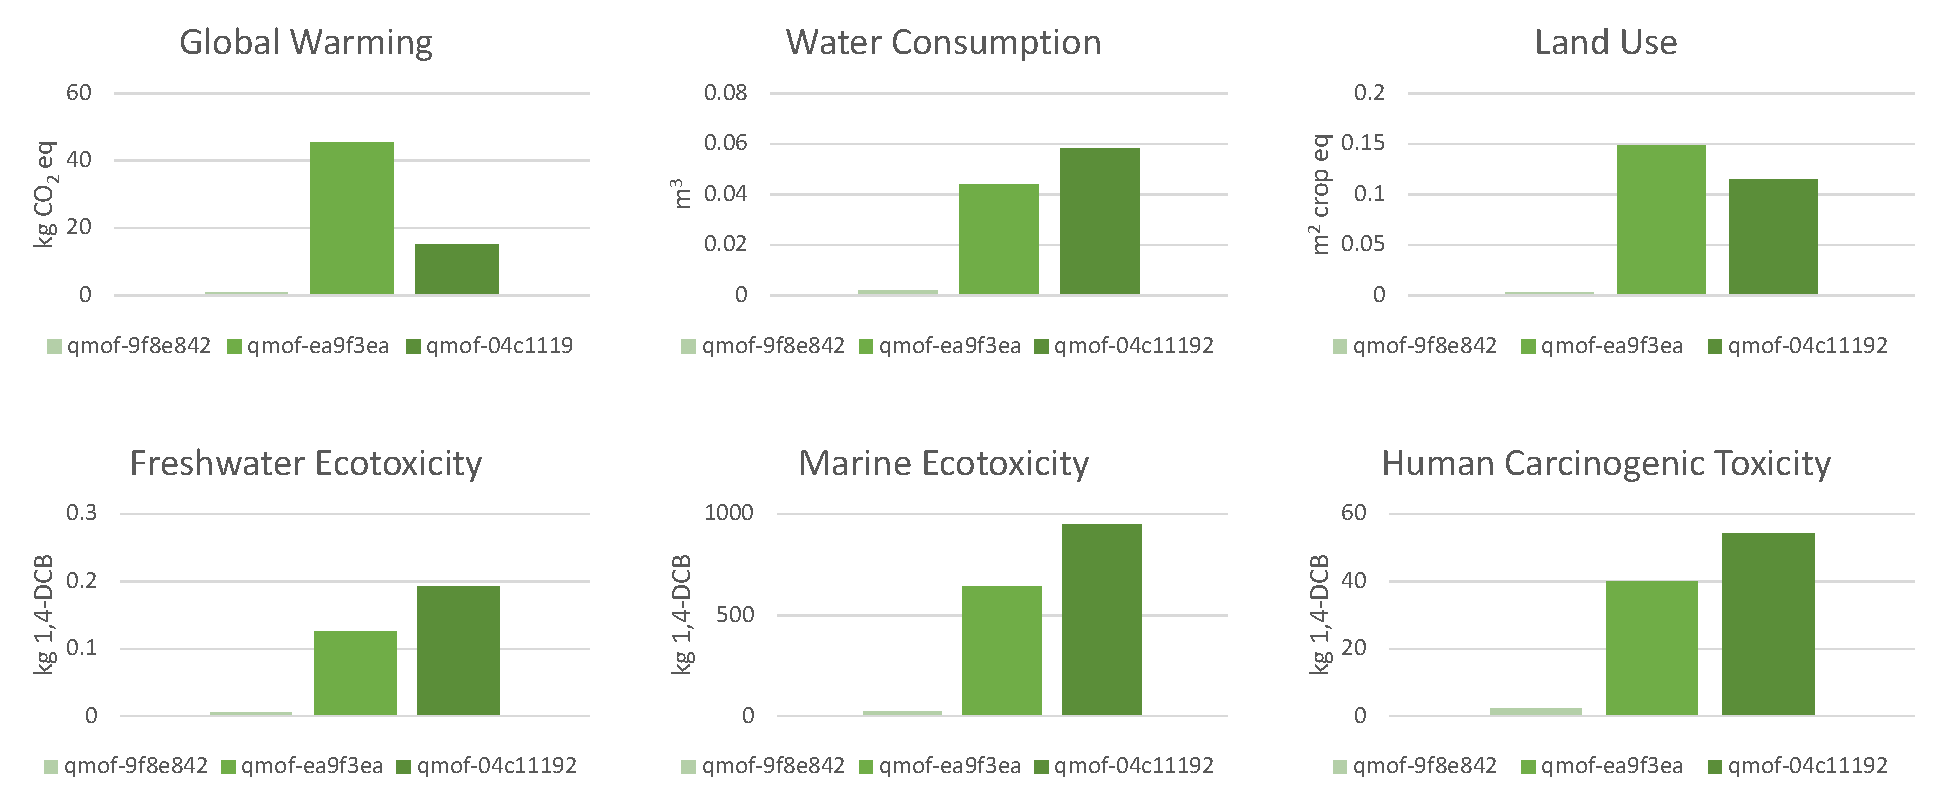
\includegraphics[height=8cm]{figure6d.pdf}
 \caption{Life-cycle analysis of qmof-04c1119, qmof-ea9f3ea, and qmof-9f8e842. Material precursors were analyzed using Simparo 10.1 to show each materials impact on critical categories such as global warming, ecotoxicity, and water consumption.}
 \label{fgr:example2col}
\end{figure*}

\section{Discussion}

The final results from the computational screening along with MC and LCA analysis show 8 highly attractive materials, 3 of which have been experimentally synthesized and 5 which have only been designed computationally.  Table 1 shows the overall materials that had passed the screenings:



\par

Of the 3 synthesized materials, the top choice based on the MC and LCA analysis is qmof-9f8e842, also known as Mg-MOF-74\cite{rosi_rod_2005}. Additionally, qmof-ea9f3ea is the Nickel variant of MOF-74. These are a well studied material used for gas adsorption and CO\textsubscript{2} conversion by photocatalysis and hydrogenation\cite{adhikari_mg-mof-74_2025, yang_co2_2012, britt_highly_2009, yasumura_co2_2025, stolar_scalable_2021, zurrer_mixed-metal_2021, dong_ligand_2024}. This material being included gives confidence in the screening method to find highly suitable materials for CO\textsubscript{2} conversion. Several in-silico studies have been done on MOF-74: Adhikari et al\cite{adhikari_silico_2025} ran calculations looking at CO, CO\textsubscript{2}, and CH\textsubscript{4} on the Mg, Zn, and Cu variants of MOF-74. The results pointed to favorable CO\textsubscript{2} binding energies, with the Mg variant allowing for the highest CO\textsubscript{2} adsorption capacity at 10.9 mmol/g. 
\par
McCarver et al\cite{mccarver_catalyst_2023} conducted a comprehensive DFT analysis to understand the reaction mechanism and competing pathways for the CO\textsubscript{2} to CH\textsubscript{4} reaction using X-MOF-74 (X = Mg, Mn, Fe, Co, Ni, Cu, Zn). Even with variations in their computational method, their analysis further supported our DFT calculations showing that Mg-MOF-74 would thermodynamically support "CO\textsubscript{2} to CH\textsubscript{4} due to favorable interactions of reduced CO\textsubscript{2} intermediates with the open-metal site". Their actual calculations however suggest that Mg-MOF-74 kinetically would favor H\textsubscript{2} production and may form diverse products (intermediates) along the way to CH\textsubscript{4}. 
\par
Lastly, we look at experimental work conducted by Yasumura et al\cite{yasumura_co2_2025}, who investigated CO\textsubscript{2} hydrogenation over Mg, Ni, and Mg/Ni-MOF-74 catalysts. At 350\textdegree C their results share that Mg-MOF-74 was the only material to be stable under the reaction conditions, with x-ray diffraction patterns retained. This agrees with the ML thermal prediction of Ni-MOF-74 decomposing at 325\textdegree C while Mg-MOF-74 is able to remain stable up to 371\textdegree C. While Ni-MOF-74 showed worse stability, its CO\textsubscript{2} conversion rate remained several times higher than Mg while the catalyst was active. Through combination of the two catalysts, they found that use of a more highly active catalyst (Ni nanoparticles) dispersed within the Mg-MOF-74 framework achieved 35\% CO\textsubscript{2} conversion with 80\% selectivity for CH\textsubscript{4} at 350\textdegree C with the structure remaining intact after 50 hours of continuous use. Future work can look at the stability of Ni-MOF-74 at lower temperatures. These results support the material as being a suitable material to host superior catalysts at high dispersion. 

\par

The third material qmof-04c1119, or Zn-IRMOF-10, also has had several studies with looking at the materials CO\textsubscript{2} adsorption ability\cite{yang_ab_2012, yang_porous_2020}. Borycz et al\cite{borycz_co2_2016} ran a computational study on M-IRMOF-10 (M = Mg, Ca, Fe, Cu, Zn, Ge, Sr, Cd, Sn, and Ba) CO\textsubscript{2} adsorption at high and low pressures. The Zn variant performed well reaching up to 52mol/kg at 50 bar. their binding energy calculations show 18kJ/mol, while not the best of the metal nodes tested, Zn's availability competes with the better performing rare earth elements. While there is limited experimental work done directly on CO\textsubscript{2} hydrogenation or photo-reduction, this computational work and stability from experimental work focused on other uses gives confidence in the materials application in CO\textsubscript{2} conversion. 

The materials of high interest are the MOFs that have not been experimentally synthesized and tested yet. Four of the materials were generated from the Boyd and Woo dataset\cite{burner_arcmof_2023}, and one was developed by Lan et al.\cite{lan_large-scale_2019} in the Genomic MOF dataset. The Boyd and Woo dataset was curated from a 300,000 MOFs looking at materials that could show strong CO\textsubscript{2} binding sites and can capture CO\textsubscript{2} in wet flue environments. The Genomic MOF dataset performed computational assembly of 550,357 MOFs, then performed configurational-bias Monte Carlo simulations looking at materials that can perform CO\textsubscript{2} capture. 

\par
\begin{table*}
\small
  \caption{\ Passing material lists with qmof identification that can be used to search for the material on Materials Project\cite{jain_commentary_2013}; Band gap data shows QMOF band gap + 0.85 eV\cite{fumanal_charge_2020}}
  \label{tbl:example2}
  \begin{tabular*}{\textwidth}{@{\extracolsep{\fill}}lllllll}
    \hline
    
    qmof ID & Chemical Formula & Porosity [{\AA}] & Thermal Breakdown Temp (C^{\circ}) & Estimated Band Gap [eV] & Synthesized
    \\
    \hline
    qmof-04c1119	&Zn\textsubscript{12}C\textsubscript{216}H\textsubscript{136}N\textsubscript{16}O\textsubscript{48}	&	4.8&	371.5	&2.58	&YES\\

    qmof-ea9f3ea	&Ni\textsubscript{6}C\textsubscript{24}H\textsubscript{6}O\textsubscript{18}&10.4&	325.7	&1.30	&YES\\

    qmof-9f8e842	&Mg\textsubscript{6}C\textsubscript{36}H\textsubscript{12}O\textsubscript{18}&	15.3&	397.8	&2.62&	YES\\

    qmof-0e64acd	&Al\textsubscript{6}C\textsubscript{100}H\textsubscript{51}N\textsubscript{7}O\textsubscript{36}&	5.0	&292.0	&1.30	&NO\\ 
    
    qmof-52ef7e9	&Al\textsubscript{2}C\textsubscript{42}H\textsubscript{24}N\textsubscript{6}O\textsubscript{12}&21.6&	247.7	&2.46&	NO\\ 

    qmof-91692c9&	Al\textsubscript{6}C\textsubscript{84}F\textsubscript{30}H\textsubscript{8}O\textsubscript{28}	&	5.9	&365.6	&2.62&	NO\\

    qmof-07c07d3&	Zn\textsubscript{6}C\textsubscript{76}H\textsubscript{60}O\textsubscript{50}&	5.5	&367.9	&2.58&	NO\\

    qmof-74ace65&	Zn\textsubscript{4}C\textsubscript{44}Cl\textsubscript{14}F\textsubscript{14}H\textsubscript{6}N\textsubscript{16}&	4.7	&322.9	&3.31&	NO\\

  \hline
  \end{tabular*}
\end{table*}

\begin{figure}[h]
\centering
  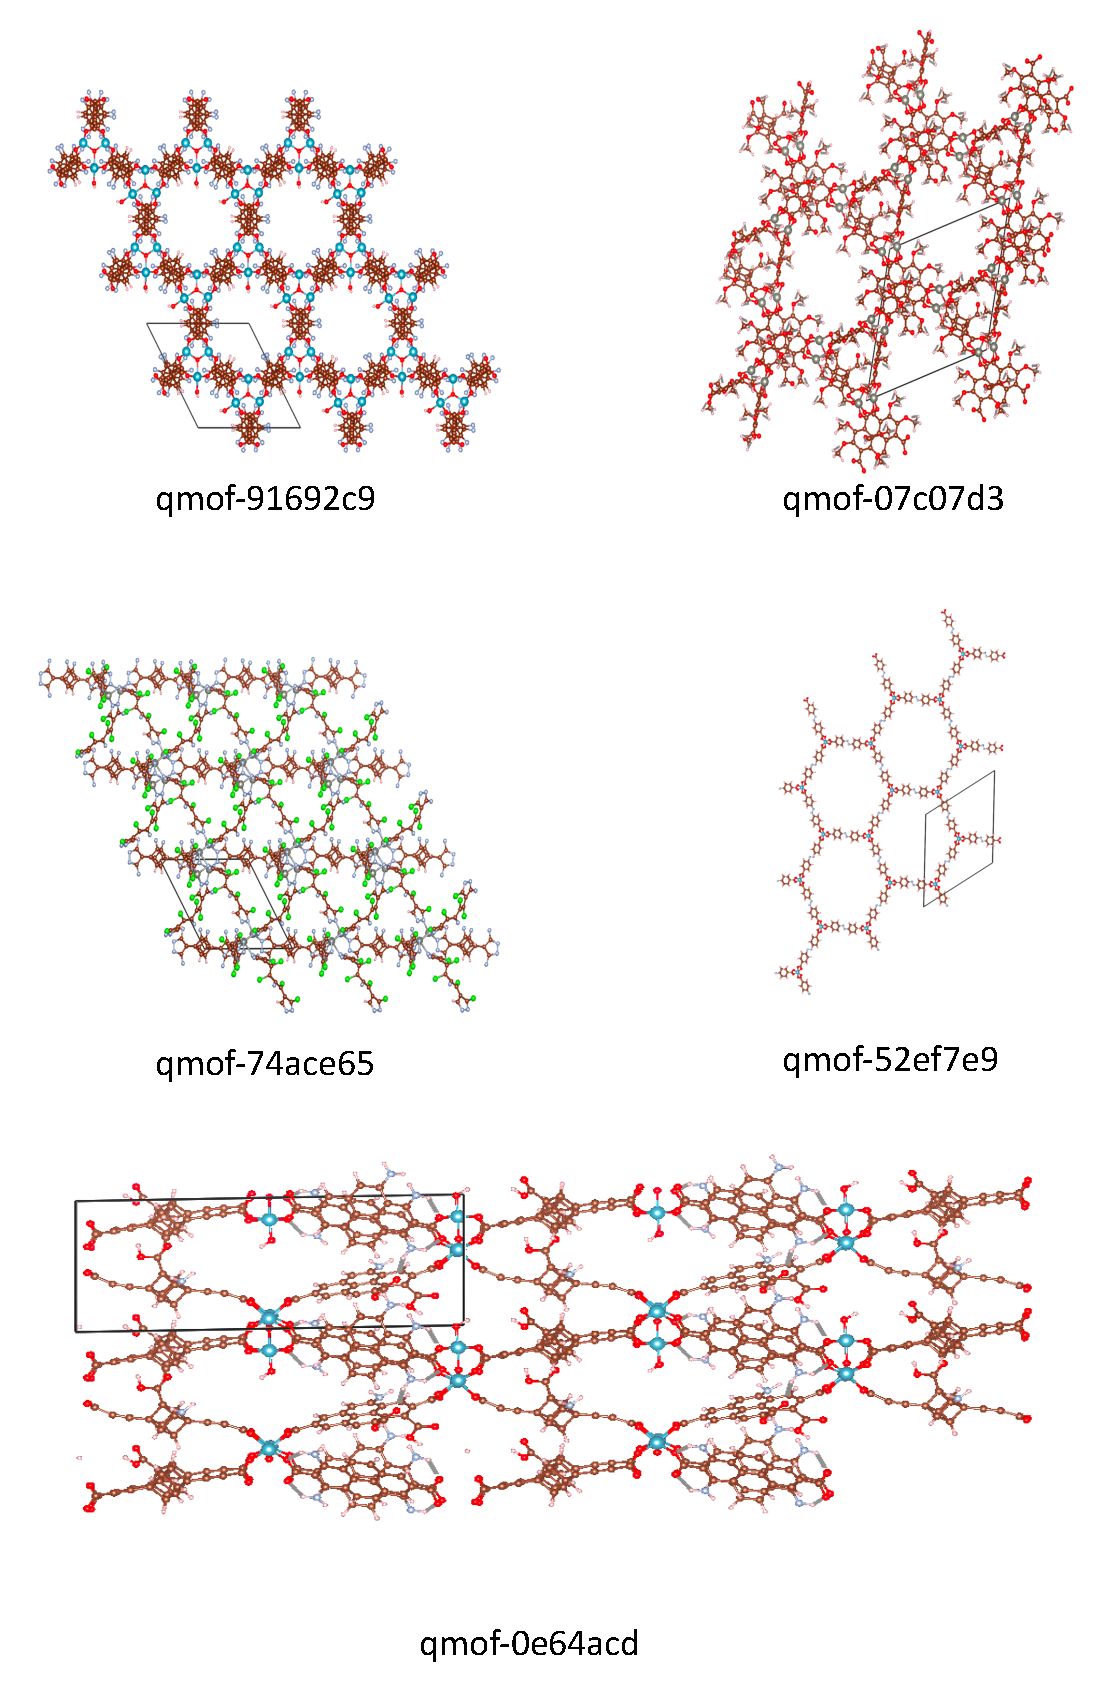
\includegraphics[height=10cm]{figure7b.pdf}
  \caption{Crystal structures of the five metal-organic frameworks that have not been experimentally realized. Structures were sourced from the Boyd \& Woo and Genomic MOFs databases via the QMOF Database. All five feature carboxylate-coordinated metal nodes with nitrogen- or halogen-functionalized linkers, and span pore-limiting diameters from 4.7 to 21.6 Å.}
  \label{fgr:example}
\end{figure}
Of the theoretical passing MOFs, three are aluminum-based frameworks (qmof-0e64acd, qmof-52ef7e9, and qmof-91692c9) and two zinc-based frameworks (qmof-07c07d3 and qmof-74ace65). Of these materials, qmof-52ef7e9 presents a simpler synthesis pathway than the other materials. The azobenzene dicarboxylic acid linker is available commercially\cite{noauthor_azobenzene-44-dicarboxylic_nodate} and links with the aluminum metal nodes in a ttp topology. The large pore size of the material, 21.59 Angstrom, should provide ample room for CO\textsubscript{2} adsorption while letting converted products pass through the pores. The azobenzene linker has also shown light adsorption which can aid in a light-assisted photo-hydrogenation reaction\cite{wang_photoswitching_2015}. The other two aluminum materials organic linkers are more complex, most likely requiring multi-step synthesis reactions, increasing cost and energy required for production. The zinc-based materials show similar synthesis requirements with qmof-07c07d3 features a zinc paddle-wheel in an nbo topology, similar to more researched materials such as HKUST-1. The MOF qmof-74ace65 forms a hex topology with pyrazole-based linkers, which should allow for stable synthesis of the material.


\section{Conclusions}

In this work, we applied a multi-tiered high-throughput screening methodology to identify metal-organic frameworks suitable for CO\textsubscript{2} photo-hydrogenation. 20,375 materials were filtered for their porosity, band gap, aqueous stability, and synthesis stability. The passing materials were then computationally screening using DFT analysis of the reaction energies to find 8 highly attractive materials. Material cost analysis and life-cycle analysis were conducted to find the price per gram of each material along with the environmental impacts of the previously synthesized materials to find qmof-9f8e842 (Mg-MOF-74) offers the most favorable profile. The LCA analysis showed the impact that green solvent makes on environmental harm when comparing MOFs with similar ligands yet slight different synthesis pathways. Of the theoretical materials that have not been experimentally realized, qmof-52ef7e9 emerged as an attractive material due to its potentially easy synthesis pathway, along with its high porosity and light adsorption properties. While the QMOF database was used here, further work could explore other large database's such as MOFX-DB\cite{bobbitt_mofx-db_2023} built with the full CoRE MOF DB\cite{chung_advances_2019}, h-mof\cite{wilmer_large-scale_2012}, and ToBBaC0\cite{colon_topologically_2017} databases, expanding the total number of starting materials. This study reduces the thousands of potential MOFs that could be synthesized for CO\textsubscript{2} reduction and presents 5 highly attractive materials for novel experimental research. 

\section*{Author contributions}
MK: Methodology, Software, Writing - Original Draft \& Review and Editing. ALCM: Conceptualization, Formal Analysis, Writing - Review and Editing. TH: Project Administration, Supervision, Funding Acquisition, Writing - Review and Editing.      

\section*{Conflicts of interest}
There are no conflicts to declare.

\section*{Data availability}
Information on the DFT, TEA, and LCA analysis are provided in the Supporting Information.
The code repository containing the high-throughput scripts, DFT input and output files, and MC/LCA analysis has been archived at \textbf{MATERIALCLOUDLINK} and https://github.com/MoinKhwaja/HTS\_MOF\_Hydrogenation. The QMOF database is available at https://github.com/Andrew-S-Rosen/QMOF.

\section*{Acknowledgements}

This study was carried out using the TSUBAME4.0 Supercomputer at Institute of Science Tokyo.

%%%END OF MAIN TEXT%%%

%The \balance command can be used to balance the columns on the final page if desired. It should be placed anywhere within the first column of the last page.

\balance

%If notes are included in your references you can change the title from 'References' to 'Notes and references' using the following command:
%\renewcommand\refname{Notes and references}

%%%REFERENCES%%%
\bibliography{references.bib} %You need to replace "rsc" on this line with the name of your .bib file
\bibliographystyle{rsc} %the RSC's .bst file
\end{document}
